\chapter{Methods}
\label{sec:methods}

\section{Spiking network simulation}
\label{subsec:methods_simulation}
Following \citeauthor{nordlie2009}'s.~\cite{nordlie2009} suggestions on 
"good model description practice",
the network model is described in detail in the following paragraphs while a detailed 
overview is provided in two tables: The model is summarized in Table 
\ref{tab:model_description}, 
whereas specific numerical values of the parameters are shown in Table 
\ref{tab:network_params}. 

%\subsection{Model composition and connectivity}
% Model description

\begin{table}[tb]
    \myfloatalign
    \caption[Model description, overview]{
        Model description according to \citeb{nordlie2009}. 
        Specific parameters are shown in Table \ref{tab:network_params}.
        }
    \label{tab:model_description}
    \small
    \begin{tabular}{b{3.1cm} p{8.5cm}} \toprule
        \modelheadline{Model summary} \\
        Populations     &   8 cortical populations\\
        Topology        &   --\\
        Connectivity    &   Random connections with fixed number of synapses for 
                            each combination of pre- and postsynaptic population\\
        Neuron model    &   Leaky integrate-and-fire, fixed voltage threshold, fixed 
                            absolute refractory period\\
        Synapse model   &   Exponential-shaped postsynaptic current\\
        Plasticity      &   --\\
        Input           &   Independent fixed-rate Poisson spike trains to iaf neurons\\
        Measurements    &   Spike activity, membrane potentials \tnn

        \modelheadline{Populations} \\
        Layers          &   L2/3, L4, L5, L6 \\
        Composed of     &   One excitatory (e) and one inhibitory (i) population per layer\\
        Size            &   Population specific size \tnn

        \modelheadline{Connectivity} \\
        Type            &   Random connectivity with independently chosen pre- and postsynaptic
                            neurons; fixed total number of connections between two populations \\
        Weights         &   Fixed; drawn from clipped Gaussian distributions 
                            ($w > 0$ for excitatory, $w~<~0$ for inhibitory)\\
        Delays          &   Fixed; drawn from clipped Gaussian distributions ($d~>~0$);
                            multiples of computation step size \tnn

        \modelheadline{Neurons and synapse model} \\
        Name            &   iaf neuron\\
        Type            &   Leaky integrate-and-fire, exponential-shaped current inputs\\
        Subthreshold dynamics of neuron~$i$
                        &   {$\!\begin{aligned} 
                                \tau_\text{m} \,\dot{V_i}(t) 
                                    &= -(V_i(t) - E_\text{L}) + \frac{\tau_\text{m}}{C_\text{m}} I_i(t)
                                        &\text{if}\quad& t > t^* + \tau_\text{rp} \\ 
                                V_i(t)        
                                    &= V_\text{r}  &\text{else}& \\[0.2cm]
                                I_{\text{syn}, ij}(t) 
                                    &= w_{ij} \exp{\left(\frac{-t}{\tau_\text{syn}}\right)} \\[0.2cm]
                            \end{aligned}$}  \\
        Spiking         &   If $\,\,V_i(t_-) < \theta \quad \land \quad V_i(t_+) \ge \theta$: \\
                        &   \quad 1. set $t^* = t$    \\
                        &   \quad 2. emit spike with time stamp $t^*$ \\
        \bottomrule
    \end{tabular}
\end{table}

The network consists of eight cortical populations arranged in four 
layers. Each layer contains an excitatory as well as an inhibitory population, 
implying what is known as Dale's principle: neurons can only be of one type or the other.%
\footnote{
The actual principle is aimed at more detailed models, hence more specific stating that
"at all the axonal branches of a neuron, there was liberation of the same transmitter 
substance or substances"~\cite{eccles1976electrical}.
} %
A simplified diagram of the network together with an illustration of population 
sizes is given in Figure \ref{fig:model_description}. 
A total of 77169 leaky integrate-and-fire neurons are distributed according to the population
sizes given in Table \ref{tab:network_params}. The total numbers of excitatory and inhibitory 
neurons are 61843 and 15326, respectively, yielding a ratio of 4.04 of excitatory over inhibitory
neurons. 

\begin{figure}[tb]
    \centering 
    \begin{subfigure}[b]{0.6\textwidth} 
        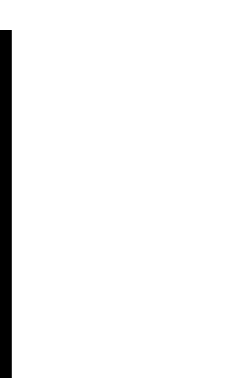
\includegraphics{../figures/diagram_colored_print}
        \label{fig:diagram}
    \end{subfigure}
    \begin{subfigure}[b]{0.35\textwidth}
        \includegraphics{\figdir population_size}
        \label{fig:population_size}
    \end{subfigure} ~
    \caption[Diagram of model and population sizes]{
        Description of the network model. 
        (\textbf{A})~% 
        Diagram of the layered cortical network. 
        Layers 23, 4, 5, and 6 are composed of one excitatory
        (triangles) and one inhibitory population (circles) each.
        The connections are only shown for probabilities $>0.04$. 
        The external input is simulated by Poissonian spike trains
        with adapted rates for each population. 
        Layer 1 does not contain neuron populations.
        (\textbf{B})
        Population sizes, total of 77169 neurons. The total number of inhibitory neurons is roughly
        $1 / 4$ of the number of excitatory neurons. 
    }
    \label{fig:model_description} 
\end{figure}
Synapses are created according to a set connection rule, referred to as 
"fixed total number":
For each combination of pre- and postsynaptic population, pairs of neurons to be connected are drawn
randomly until a fixed number of synapses is reached, 
allowing for multiple synapses and self-connections. 
Potjans and Diesmann's original model defines the connection probability $P_{\text{conn}, \,ab}$ 
of one neuron in the presynaptic population $a$ to form at least one connection with one neuron in 
the postsynaptic population $b$. For given population sizes $N_a$ and $N_b$, the number of 
synapses $C_{ab}$ is then calculated by
\begin{equation}
    C_{ab} = \frac{\ln \left( 1 - P_{\text{conn}, \,ab} \right)}{\ln \left( 1 - \frac{1}{N_a N_b} \right)} \, ,
    \label{eq:synapse_numbers}
\end{equation}
the inverse of the formula for connection probabilities of the original study~\cite{potjans2014}.

The weight $w$ for each synapse is drawn from a normal distribution.
For excitatory presynaptic neurons, this mean value is set to $87,8$ pA (see below for 
a derivation). The mean for inhibitory ones is determined by multiplying 
with a factor $-g$, where the relative inhibitory synapse strength is set to 
$g = 4$. There is one important exception to this scheme:
The mean for the connection from L4e to L2/3e is increased by a factor of 
$j_{02} = 2$ (consult \cite{potjans2014} for details). 
The standard deviation is set to $10\%$ of the mean. 
The distributions from which weights are drawn are clipped, 
such that a neuron assigned to the excitatory 
population will not have associated outgoing synapses with $w < 0$ 
and vice versa for inhibitory ones. 
Delays are drawn from normal distributions as well, with a mean value 
of $1.5$ ms for excitatory presynaptic neurons and half this value for 
inhibitory ones. The relative standard deviation is set to $50 \%$. The distributions
are again clipped such that $d \ge 0$

%\subsection{Neuron and synapse model}
The neurons are leaky integrate-and-fire neurons with a fixed voltage threshold. 
Below the threshold $\theta$, the dynamics of the membrane potential $V_i(t)$ 
for neuron $i$ are governed by the differential equation 
\begin{equation}
    \tau_\text{m} \,\frac{\text{d} V_i(t)}{\text{d} t} 
            = -(V_i(t) - E_\text{L}) + \frac{\tau_\text{m}}{C_\text{m}} I_i(t) \, .
    \label{eq:leaky_integrator}
\end{equation}
The membrane is specified by its resting potential $E_\text{L}$, 
its time constant $\tau_\text{m}$ and the capacitance $C_\text{m}$.
If, at time $t$, the threshold is reached, the neuron emits a spike and remains 
in a refractory period for a fixed time $\tau_\text{rp}$, with the membrane 
potential set to $V_\text{r}$ and discarding any input arriving. 
The total input to the neuron is represented by 
the current $I_i(t)$, which is a linear superposition of the individual 
postsynaptic currents (PSC) of the recurrent network.

The model implements  
postsynaptic current synapses with exponential shape, such that each 
spike arriving at one neuron leads to a current 
\begin{equation}
I_{\text{syn}}(t) = w \exp{\left(\frac{-t}{\tau_\text{syn}}\right)}	
    \label{eq:synaptic_current}
\end{equation}
where $w$ is the weight of the synapse in the model,
which corresponds to the amplitude of the PSC
at the time the spike arrives. 
$\tau_\text{syn}$ is the synaptic time constant.
Since measuring currents remains a difficult task for experimentalists, 
the model relays on measurements of the amplitude of the postsynaptic 
potential (PSP). In order to use the experimental observations,
an approximative transformation is implemented.
The PSC induced by one spike of given PSP with the membrane potential
at rest is calculated as follows:
For $E_\text{L} = 0$, setting $I(t) = I_\text{syn}(t)$ in equation \eqref{eq:leaky_integrator}
yields:
\begin{equation}
    \dot{V}(t)
    = - \frac{1}{\tau_\text{m}} V(t) + \frac{w}{C_m} \exp{\left(-\frac{t}{\tau_\text{syn}}\right)} \,.
    \label{eq:psc_ode}
\end{equation}
This has the solution 
\begin{equation}
    V(t) =   
        - \frac{w \tau_\text{m} \tau_\text{syn}} {C_\text{m} \left(\tau_\text{m} - \tau_\text{syn}\right)}	
        \exp{\left( -\frac{t}{\tau_\text{syn}} \right)} 
        + C_1 \exp{\left(-\frac{t}{\tau_\text{m}} \right)}
    \label{eq:psc_ode_sol}
\end{equation}
with integration constant $C_1$.
With the boundary condition $V(t = 0) = 0$, this constant is set to
\begin{equation}
    C_1 = \frac{w \tau_\text{m} \tau_\text{syn}}{C_\text{m} \Delta\tau}	
    \label{eq:C_1}
\end{equation}
where $\Delta\tau := \tau_\text{m} - \tau_\text{syn}$ is introduced.
Thus
\begin{equation}
    V(t) = C_1 \left[\exp\left(-\frac{t}{\tau_\text{m}}\right) - \exp\left(-\frac{t}{\tau_\text{syn}}\right)\right]	\,.  
    \label{eq:V(t)}
\end{equation}
In order to get the peak PSP, we search for the maximum. Setting $\dot{V}(t) = 0$ 
yields
\begin{equation}
    t_\text{max} 
        = \ln{\!\left(\frac{\tau_\text{syn}}{\tau_\text{m}}\right)} 
            \left(\frac{1}{\tau_\text{m}} - \frac{1}{\tau_\text{syn}}\right)^{-1} \,.
    \label{eq:t_max}
\end{equation}
Inserting into equation \eqref{eq:V(t)} leads to 
\begin{equation}
    V(t_\text{max}) 
        = \frac{w \tau_\text{m} \tau_\text{syn}}{C_\text{m} \Delta\tau}	
            \left[ 
                \left( \frac{\tau_\text{syn}}{\tau_\text{m}} \right)^\frac{\tau_\text{syn}}{\Delta\tau} 
            - \left( \frac{\tau_\text{syn}}{\tau_\text{m}} \right)^\frac{\tau_\text{m}}{\Delta\tau} 
            \right] \,.
    \label{eq:PSP}
\end{equation}
For a given PSP amplitude, this equation is simply inverted in order to get the according 
weight $w$. The value used for the original model and also applied in this work 
is 0.15 mV. It is suggested by experiments and yields 
a synaptic weight of 87.8 pA. 
Finally, the 
input current of neuron $i$ can be described as the sum over currents induced by
arriving spike trains, 
\begin{equation}
    I_i(t) = \sum_j w_{ij} \sum_k \exp\left(\frac{t - t_j^k - d_{ij}}{\tau_\text{syn}}\right) \, ,
    \label{eq:input_current}
\end{equation}
where $t_j^k$ is the time the $k$-th spike by neuron $j$ was emitted and the 
delay between neuron $i$ and $j$ is set to $d_{ij}$. 

%\subsection{Model input, output and free parameters}
The activity of the network depends both on the recurrent stimulation as well as 
external input. The biological networks motivating the model are shown to be 
stable under a wide range of conditions\emph{CITE}. 
The inhibitory populations that guarantee this stability require that the network 
is supplied with external stimuli -- without this, it converges to quiescence.\cite{brunel2000}
In the case of the local neocortical microcircuit, the roles of different
external input and recurrence is debated widely. While some interpret the local circuit
as computational building blocks \cite{potjans2014}, others focus on the interplay between 
different cortical regions (e.\,g. \citeb{boucsein2011beyond}) or the transmission of 
thalamic signals (\emph{CITE}). The model implemented in this work is only driven 
by unspecific input mimicking stimulation from close and distant cortical areas\cite{potjans2014}.%
\footnote{
The original publication included thalamic input in order to examine temporal transmission 
of stimuli. This is omitted here as the focus lies on stationary states. 
}

Instead of using simulated neurons populations, the input is implemented as Poissonian 
spike trains. The underlying Poisson process with mean rate $\nu$ is a stochastic process formally 
defined as a continuous-time counting process ${N(t), t \le 0}$ with the properties%
~\cite{tuckwell2005introduction}
\begin{itemize}
    \item $N(0) = 0$;
    \item for any $0 = t_0 < t_1 < t_2 < \cdots < t_{n-1} < t_n$, the random variables
        $N(t_k) - N(t_{k-1}), k = 1, 2, \dots, n$ are mutually independent; 
    \item for any $0 \le t_1 < t_2, N(t_1) - N(t_2)$ is a Poisson random variable with 
        probability distribution 
        \begin{equation}
            \text{Pr}\left\{N(t_2) - N(t_1) = k \right\} 
                = \frac{\left( \nu(t_2 - t_1) \right)^k \exp \left( - \nu(t_2 - t_1) \right) }{k!}
            \label{eq:poisson_process}
        \end{equation}
        for $k \in \mathbb{N}$.
\end{itemize}
For the random variable $N(t_2) - N(t_1)$, mean and variance are given by
$\text{E}[N(t_2) - N(t_1)] = \text{Var}(N(t_2) - N(t_1)) = \nu(t_2 - t_1)$,
such that the average number of spikes $\langle k \rangle$ 
per time bin of width $\Delta t = t_2 - t_1$ is 
\begin{equation}
    \frac{\langle{N}\rangle}{\Delta t} = \nu \,.
    \label{eq:poisson_rate}
\end{equation}
Furthermore, as mean and variance for the Poisson process are equal, the often cited 
Fano factor
\begin{equation}
    F = \frac{\sigma^2}{\mu}\,,
    \label{eq:Fano}
\end{equation}
defined for a random process with mean $\mu$ and variance $\sigma$, 
is equal to one. 

In the spiking network model, each neuron receives spikes of a defined weight with 
the spike times implemented as such a Poisson process. All processes are mutually independent 
and the rate of each one is determined by a global 
background rate of $8$ Hz multiplied by an external indegree $(C_\text{ext})_a$ for
population $a$. 
This mimics a multiple number of synapses to the respective neuron, each receiving an 
independent Poisson process with a mean rate of $8$ Hz. 

At creation, the neurons are initialized by drawing their membrane potential from a normal
distribution with mean $-58$ mV and a standard deviation of $10$ mV. 
The activity of the network is measured in terms of spike trains (measuring the spike times 
of single neurons up to the maximal grid resolution $h$) and membrane potentials in mV. 
The results in this thesis are based on recording only a fraction of the neurons in the network, 
choosing $n_a$ random neurons of each population $a$. 
If not specified else, spikes are recorded 
from $1000$ neurons of each population, membrane potentials from $100$. The further analysis of the data 
is explained in following sections.
The large number of free parameters of the model and their chosen values are summarized in 
Table \ref{tab:network_params}. 
% Network parameters
\begin{table}[tb]
    \centering
    \caption[Network parameters]{
        Network parameters
        }
    \label{tab:network_params}
    \small
    \begin{tabular}{p{2.2cm}| *{8}{x{0.9cm}}} \toprule
        \paramsheadline{Populations and input} \tn 
        Layer 
        & \mc2c{L2/3} & \mc2c{L4} & \mc2c{L5} & \mc2c{L6}  \tn
        Population& \mc1c{e} & \mc1c{i} & \mc1c{e} & \mc1c{i} & \mc1c{e} & \mc1c{i} & \mc1c{e} & \mc1c{i} \tn \hline
        %& L2/3e & L2/3i & L4e & L4i & L5e & L5i & L6e & L6i  \tn \hline
        Pop. size, $N_a$   
            & 20683 & 5834 & 21915 & 5479 & 4850 & 1065 & 14395 & 2948 \tn
        $(C_\text{ext})_a$ 
            & 1600 & 1500 & 2100 & 1900 & 2000 & 1900 & 2900 & 2100 \tn[0.1cm]
        Backgr. rate     
        &&&& 8 Hz \tnn

        \paramsheadline{Connection probabilities for pre- and postsynaptic populations} \tn
        \multirow{2}{*}{\diagbox[width=2.65cm]{post~~~~}{pre~~~}}
        & \mc2c{L2/3} & \mc2c{L4} & \mc2c{L5} & \mc2c{L6}  \tn
        & \mc1c{e} & \mc1c{i} & \mc1c{e} & \mc1c{i} & \mc1c{e} & \mc1c{i} & \mc1c{e} & \mc1c{i} \tn \hline
          %    &L2/3e & L2/3i & L4e & L4i & L5e & L5i & L6e & L6i  \tn \hline
        L2/3e
            & 0.101 & 0.169 & 0.044 & 0.082 & 0.032 & 0 & 0.008 & 0 \tn 
        L2/3i
            & 0.135 & 0.137 & 0.032 & 0.051 & 0.075 & 0 & 0.004 & 0 \tn 
        L4e
            & 0.008 & 0.006 & 0.050 & 0.135 & 0.007 & 0 & 0.045 & 0 \tn 
        L4i
            & 0.069 & 0.003 & 0.079 & 0.160 & 0.003 & 0 & 0.106 & 0 \tn 
        L5e
            & 0.100 & 0.062 & 0.051 & 0.006 & 0.083 & 0.373 & 0.020 & 0 \tn 
        L5i
            & 0.055 & 0.027 & 0.026 & 0.002 & 0.060 & 0.316 & 0.009 & 0 \tn 
        L6e
            & 0.016 & 0.007 & 0.021 & 0.017 & 0.057 & 0.020 & 0.040 & 0.225 \tn 
        L6i
            & 0.036 & 0.001 & 0.003 & 0.001 & 0.028 & 0.008 & 0.066 & 0.144 \tnn

        \paramsheadline{Further connectivity} \tn
        $w \pm \delta w$    
            &  \multicolumn{3}{l}{$87.8 \pm 8.8 \,\text{pA}$}
            &  \multicolumn{5}{l}{Excitatory synaptic strengths} \tn
        $j_{02}$    
            &  \multicolumn{3}{l}{$2$}
            &  \multicolumn{5}{l}{Factor for connection L4e $\to$ L2/3e} \tn
        $g$    
            &  \multicolumn{3}{l}{$4$}
            &  \multicolumn{5}{l}{Relative inhibitory synapse strength} \tn
        $d_e \pm \delta d_e$    
            &  \multicolumn{3}{l}{$1.5 \pm 0.75 \,\text{ms}$}
            &  \multicolumn{5}{l}{Excitatory synaptic transmission delays} \tn
        $d_i \pm \delta d_i$    
            &  \multicolumn{3}{l}{$0.8 \pm 0.4 \,\text{ms}$}
            &  \multicolumn{5}{l}{Inhibitory synaptic transmission delays} \tnn

        \paramsheadline{Neuron model} \tn
        $\tau_\text{m}$    
            &  \multicolumn{3}{l}{$10 \,\text{ms}$}
            &  \multicolumn{5}{l}{Membrane time constant} \tn
        $\tau_\text{ref}$    
            &  \multicolumn{3}{l}{$\hphantom{0}2 \,\text{ms}$}
            &  \multicolumn{5}{l}{Absolute refractory period} \tn
        $\tau_\text{syn}$    
        &  \multicolumn{3}{l}{$\hphantom{0}0.5 \,\text{ms}$}
            &  \multicolumn{5}{l}{Postsynaptic current time constant} \tn
        $C_\text{m}$    
            &  \multicolumn{3}{l}{$250 \,\text{pF}$}
            &  \multicolumn{5}{l}{Membrane capacity} \tn
        $E_\text{L}$    
            &  \multicolumn{3}{l}{$-65 \,\text{mV}$}
            &  \multicolumn{5}{l}{Leaky rest potential} \tn
        $V_\text{r}$    
            &  \multicolumn{3}{l}{$-65 \,\text{mV}$}
            &  \multicolumn{5}{l}{Reset potential} \tn
        $\theta$    
            &  \multicolumn{3}{l}{$-50 \,\text{mV}$}
            &  \multicolumn{5}{l}{Fixed firing threshold} \tn \bottomrule
    \end{tabular}
\end{table}

%\subsection{Model validation}
\begin{figure}[tb]
    \centering
    \includegraphics{\figdir syn_numbers}
    \caption[Connection between populations]{
        Connection between populations.
        (\textbf{A}) Calculated total synapse number between a pre- 
        and a postsynaptic population. These numbers are used for connecting the network, 
        using the connection rule "fixed total number". (\textbf{B}) Mean number of synapses
        a neuron in a specific postsynaptic population is receiving from all neurons of a 
        presynaptic population. These numbers are only applied when using the connection
        rule "fixed indegree" (\emph{see section comparison for details}).
    }
    \label{fig:syn_numbers}
\end{figure}
In order to verify that the model behaves reasonably, a number of basic parameters 
is examined before stating more central results. As the implementation of the neuron model
is part of the NEST software and thus well established, the validation starts at the level 
of connections. Figure \ref{fig:syn_numbers} shows the number of synapses for each pair 
of pre- and postsynaptic population and 
the mean number of synapses each neuron receives from a specific population. The total number 
of synapses in the model is almost 0.3 billion synapses.  

With the connection rule "fixed total number" applied in the simulation, 
the number of synapses per postsynaptic neuron is expected to follow a binomial distribution:
For pre- and postsynaptic populations $a$ and $b$, respectively, 
each time a pair is drawn, one postsynaptic neuron is chosen with a probability 
$1 / N_b$, $N_b$ being the population size. This is repeated until $C_{ab}$ synapses are
created. 
Choosing one neuron the first $k$ times and not again has the probability 
$\text{Pr}\left\{X = k\right\} = 
\left( \frac{1}{N_b} \right)^{k} 
\left( 1 - \frac{1}{N_b} \right)^{C_{ab} - k}$.
Multiplied by the number of possibilities to choose this neuron $k$ times out of 
$C_{ab}$, the total probabilities of receiving $k$ synapses from population $a$ is
given by
\begin{equation}
    \text{Pr}_{\,\text{Binom}}\left\{X = k; n=C_{ab}, p=\frac{1}{N_b}\right\} = 
        {C_{ab}\choose{k}} 
        \left( \frac{1}{N_b} \right)^{k} 
        \left( 1 - \frac{1}{N_b} \right)^{C_{ab} - k} \,.
    \label{eq:binomial}
\end{equation}
Accordingly, the expected value of $k$ is $\text{E}[k] = C_{ab} / N_b$, its variance is 
$\text{Var}(k) = C_{ab} (1 - 1/N_b) / N_b$. 
In Figure \ref{fig:syn_numbers_distribution}, the actual distribution of synapse numbers 
for the connection L6e $\to$ L6i is shown in a normalized histogram. 
The measured mean and standard deviation are $(975 \pm 31)$ compared to the theoretical 
value of $(979 \pm 31)$ synapses. 
Thus, the agreement between the numbers from the simulation and the theoretical expectation is
in full agreement. 
\begin{figure}[tb]
    \centering
    \includegraphics{\figdir syn_numbers_distribution}
    \caption[Distribution of synapse numbers]{
        Distribution of synapse numbers for the connection L6e $\to$ L6i.
        The total number of synapses for this connection is $2,888,426$, 
        the mean number for each neuron in L6i is $979$.
        The steps indicate the normalized histogram (bin width = 10) obtained 
        from a simulation, the dashed line is a binomial distribution, the 
        underlying distribution for the given connection rule. 
    }
    \label{fig:syn_numbers_distribution}
\end{figure}

To further validate the model on a basic level, a look at a single neurons' membrane potentials 
is taken. Figure \ref{fig:single_membrane_potential} shows the membrane 
potentials of two neurons over the first 1.2 s of simulation together with a comparison of
the normalized histograms of a larger subset of the 
respective population. The neuron of the upper plots appertains to the population
L6e, the other one to population L6i. 
Observing the first 100 ms of the membrane potential 
indicates that the used initialization leads to a large hyperpolarization at least in these two 
sample neurons. Thus, for the further analysis, a transient period of 0.2 seconds is cut off the
data before further analysis. For the remaining time, the membrane potentials fluctuate 
in a reasonable range with mean between resting potential $E_L = -65$ mV and threshold $\theta = -50$ mV, 
hitting the threshold as small number of times. 
Potjans and Diesmann state that
these two populations have comparably low / high rates, the excitatory one firing at 
$\sim 1$ Hz, the inhibitory one at $\sim 7$ Hz~\cite{potjans2014}, 
but linking this to the membrane potential distribution can be very misleading:
Rare but large fluctuations can lead to high number of spikes without substantially 
raising the average. 
Furthermore, it is can be seen, that a single 
neurons' membrane potential is not necessarily distributed as the population mean. 
This is due to the large variation in single neuron firing rates reported already in the 
original publication~\cite{potjans2014}. 

\begin{figure}[tb]
    \centering
    \includegraphics{\figdir single_membrane_potential}
    \caption[Exemplary membrane potentials]{
        Membrane potentials of two exemplary neurons of the populations 
        L6e (\textbf{A, C}) and L6i (\textbf{B, D}). The data is taken from 
        a simulation of 1.2 s, recording the membrane potential every 1 ms.
        For the histograms, the first 0.2 s are discarded. 
        In all four plots, the threshold $\theta = -50$ mV is indicated by a dashed line, 
        the resting potential $E_L = -65$ mV by a line of dashes and dots. 
        \quad (\textbf{A, B}) Membrane potential over the time of simulation. 
        The upper membrane potential reaches $\theta$ once at $t = 0.06$ s, 
        the lower one does not spike over the time recorded. 
        The initial membrane potential 
        is drawn from a normal distribution.
        \quad (\textbf{C, D}) Normalized histograms of membrane potentials of the
        two neurons (thin steps) as well as the averaged ones for a subset of $100$ 
        neurons (thick steps). 
        Note that contributions due to neurons being in refractory 
        period after spiking are not removed, yielding peaks at $V_\text{r} = -65$ mV. 
    }
    \label{fig:single_membrane_potential}
\end{figure}



\FloatBarrier
\section{Mean field model}
The derivation of a mean field theory goes along the 
lines of the work by \citeb{brunel2000}.
It starts of with a simplified model of 
$N$ leaky integrate-and-fire neurons in two populations. 
Each neuron receives input from the network by $C$ synapses, 
$C_E$ from excitatory and $C_I$ from inhibitory ones. 
Furthermore, each neurons receives $C_\text{ext} = C_E$ connections from 
external excitatory neurons.
The synapse numbers 
are determined by the relative size of the two populations through the factor
\begin{equation}
    \epsilon := \frac{C_E}{N_E} = \frac{C_I}{N_I} \,.
    \label{eq:epsilon}
\end{equation}
A central assumption is the sparsity of the network, expressed by $\epsilon \ll 1$.
Guided by anatomical estimates for the neocortex, the population sizes are set to
$N_e = 0.8N$ excitatory and $N_i = 0.2N$ inhibitory neurons. Taking the definition
\eqref{eq:epsilon}, this implies 
\begin{equation}
    C_I = \gamma C_E 	
 \label{eq:C_I}
\end{equation}
with $\gamma = 0.25$. The synaptic weights in this model are set to $J$ for 
excitatory presynaptic neurons and to $-g\, J$ for inhibitory ones, 
whereas the delays are fixed to $d$ for all synapses. 

At the heart of the mean field model
is the transition from the deterministic description of membrane potential 
dynamics to a probabilistic formulation. 
As in Potjans' model, the membrane potential follows
the differential equation \eqref{eq:leaky_integrator}. The input is simplified 
by implementing voltage based synapses which
yield an instantaneous and fixed change in membrane potential
for each spike arriving at the neuron instead of an exponential shaped PSC.
It can be described by a sum over Dirac delta-functions, 
\begin{equation}
    I_i(t) = \tau_\text{m} \sum_j J_{ij} \sum_k \delta(t - t_j^k - d_{ij}) \,.
    \label{eq:input_const_volt}
\end{equation}
The synaptic weights $J_{ij}$ in this case are equal to the PSP and given in mV.  

Two important conditions have to be met in order to make the transition from 
this description to a probabilistic one:
\begin{itemize}
    \item Sparsity: This implies that 
        two neurons share only a small number of common input, such that pair correlations
        are negligible for $C / N \to 0$; 
    \item Uncorrelated input: The contributions a neuron receives have to stem from 
        a wide range of the network, each being small compared to the threshold
        (corresponding to no spatial correlations). 
        No temporal correlations imply low single neuron firing rates $\nu$ compared 
        to the membrane time constant $\tau_\text{m}$
        (e.\,g. $\nu \sim10$ Hz and $1 / \tau_\text{m} \sim 1 / (20\,\text{ms}) = 50\, \text{Hz}$).
\end{itemize}
If these conditions are met, the input can be modeled as a time-varying average part
$\mu(t)$ plus a fluctuating Gaussian part with amplitude $\sigma(t)\tau_\text{m}$:
\begin{equation}
    \frac{\tau_\text{m}}{C_\text{m}} \, I_i(t) =  \mu(t) + \sigma(t) \sqrt{\tau_\text{m}} \eta_i(t) \, .
    \label{eq:input_random}
\end{equation}
The random fluctuations are described by Gaussian white noise $\eta_i(t)$ with 
$\langle  \eta_i(t)\rangle = 0$. 
The exclusion of correlations is formalized as  
\begin{equation}
    \langle \eta_i(t) \: \eta_j(t') \rangle = \delta_{ij} \: \delta(t - t')	\, ,
    \label{eq:no_correlations}
\end{equation}
$\delta_{ij}$ corresponding to correlations between neurons, 
the Dirac delta distribution to temporal ones. 
%\emph{
    %In order to apply the mean field theory to a spiking network model, 
%the uncorrelatedness of single neurons' input has to be quantified.}

The fundamental parameter calculated by the mean field model is the single neuron
firing rate $\nu(t)$. In this basic model, it is assumed that any neuron of either 
of the two populations sees the same input on average and thus fires with the same 
rate $\nu$. This rate is linked to the average input $\mu(t)$ by
\begin{equation}
    \begin{split}
        \mu(t)          &= \mu_l(t) + \mu_\text{ext} \\
        \text{with} \qquad \mu_l(t)        &= C_E \, J (1 - \gamma g) \nu(t - d) \tau_\text{m} \\
        \mu_\text{ext}  &= C_E J \nu_\text{ext} \tau_\text{m} \,.
        \label{eq:mu}
    \end{split}
\end{equation}
Similarly, for the amplitude of fluctuations $\sigma(t)$:
\begin{equation}
    \begin{split}
        \sigma^2(t)     &= {\sigma_l}^2(t) + {\sigma_\text{ext}}^2 \\
        \text{with} \qquad {\sigma_l}^2(t)       
                        &= C_E \, J^2 (1 + \gamma g^2) \nu(t - d) \tau_\text{m} \\
        {\sigma_\text{ext}}^2  &= C_E J^2 \nu_\text{ext} \tau_\text{m} \,.
        \label{eq:sigma}
    \end{split}
\end{equation}

%\emph{Under cortical condition: (Amit, Brunel); 
%mu and sigma relate to measurable quantities!}


Brunel then transforms equations \eqref{eq:input_random} and \eqref{eq:leaky_integrator}
into a Fokker--Planck equation describing the probability distribution of the membrane 
potential $P(V, t)$ in time: 
\begin{equation}
    \tau_\text{m} \, \frac{\partial P(V, t)}{\partial t} 
       \: = \: \frac{\sigma^2(t)}{2}  \: \frac{\partial^2 P(V, t)}{\partial V^2} 
         \: + \: \frac{\partial }{\partial V}  [(V- \mu(t)) P(V, t)] \, .
    \label{eq:fokker_planck}
\end{equation}
In the terminology of stochastic differential equations, the first term on the 
right hand side corresponds to a diffusion term originating in the fluctuations $\sigma$ 
of the input whereas the second part describes a drift due to the respective mean $\mu$ 
and the leaky quality of the neuron model. Introducing the probability current 
\begin{equation}
    S(V, t) 
    \: = \: - \frac{\sigma^2(t)}{2 \tau_\text{m}} \frac{\partial P(V, t)}{\partial V}  
        \: - \: \frac{V - \mu(t)}{\tau_\text{m}} P(V, t)
    \label{eq:prob_curr}
\end{equation}
through $V$ at time $t$ yields the continuity equation 
\begin{equation}
    \frac{\partial P(V, t)}{\partial t} \:=\: - \frac{\partial S(V, t)}{\partial V} \,.
    \label{eq:continuity}
\end{equation}

The probability distribution is subject to a number of 
constraints: Since the spiking resets neurons to $V_\text{rp} < \theta$, 
the membrane potential is always below this threshold:
$P(V, t) = 0$ for $V > \theta$. Infinite probability currents are excluded 
such that $P(V, t)$ must be continuous at any point. Specifically, 
this continuity forbids infinite spiking probabilities at the threshold $\theta$. 
The resulting constraint is 
\begin{equation}
    P(\theta, t) = 0 \,.
    \label{eq:continuity} 
\end{equation}
The probability current at the threshold is equal to the firing rate
$\nu(t)$. Inserting both $S(\theta, t) = \nu(t)$ and the above constraint into 
equation \eqref{eq:prob_curr} yields
\begin{equation}
    \frac{\partial P(\theta, t)}{\partial V}    
        = - \frac{2 \nu(t) \tau_\text{m}}{\sigma^2(t)}  \,.
\end{equation}
Neurons that fired at time $t$ exit their refractory period at 
time $t + \tau_\text{rp}$ at the reset potential $V_\text{r}$. This leads to
a difference in probability current below and above $V_\text{r}$ proportional to 
the rate of neurons firing at $t - \tau_\text{rp}$, which is expressed by
\begin{equation}
    \frac{\partial P(V_\text{r}^+, t)}{\partial V} \: -  \: \frac{\partial P(V_\text{r}^-, t)}{\partial V} 
        = - \frac{2 \nu(t - \tau_\text{rp}) \tau_\text{m}}{\sigma^2(t)} \,.
\end{equation}
Finally, $P(V, t)$ is assumed to converge sufficiently quickly to zero:

\begin{equation}
\lim_{V \to -\infty} P(V, t) = 0 \, ;
    \quad 
    \lim_{V \to -\infty} V P(V, t) = 0 \,.
\end{equation}

A stationary solution $P(V, t) = P_0(V)$ with constant 
single neuron firing rate $\nu_0$ 
satisfying the above boundary conditions is then presented:
\begin{equation}
    P_0(V) = 2 \frac{\nu_0 \tau_\text{m}}{\sigma_0} 
        \exp{\left(- \frac{(V - \mu_0)^2}{{\sigma_0}^2} \right)}
        \int_{\frac{V - \mu_0}{\sigma_0}}^{\frac{\theta - \mu_0}{\sigma_0}} \! 
            \Theta \left(u - \frac{V_\text{r} - \mu_0}{\sigma_0} \right) e^{u^2} \diff u  \,. 
    \label{eq:P_V_0}
\end{equation}
Here, $\Theta(x)$ is the Heaviside step function, i.~e. 
\begin{equation}
    \Theta(x) = \begin{cases} 1 & \text{if } x \le 0 \\ 0 & \text{else } \end{cases}  \,.
    \label{eq:heaviside}
\end{equation}
The stationary mean input and fluctuation amplitudes are obtained by inserting 
$\nu_0$ into the equations \eqref{eq:mu} and \eqref{eq:sigma}, yielding 
\begin{align}
    \mu_0 	    &= C_E J \:\tau_\text{m} [\nu_\text{ext} + \nu_0(1 - g \gamma)]  \,, \\ 
    {\sigma_0}^2 	&= C_E J^{\,2} \,\tau_\text{m} [\nu_\text{ext} + \nu_0(1 + g^2 \gamma)] \,.
    \label{eq:mu_sigma_0}
\end{align}

In order to interpret $P(V, t)$ as a probability distribution, it is required to
satisfy the normalization condition
\begin{equation}
    \int_{-\infty}^{\theta} \! P(V, t) \diff V  + p_r(t) = 1 \, ,
    \label{eq:P_V_prob}
\end{equation}
where 
\begin{equation}
    p_r(t) := \int_{t - \tau_\text{rp}}^{t} \! \nu(u) \diff u 
    \label{eq:p_r}
\end{equation}
is the probability of neurons being the in refractory period.
In the constant case, this is simply 
\begin{equation}
    p_r(t) = p_{r, 0} = \nu_0 \tau_\text{rp}  \,.
    \label{eq:p_r_0}
\end{equation}

Inserting both $P_0(V)$ and $p_{r, 0}$ into the self-consistent condition \eqref{eq:P_V_prob}
then leads to an expression for $\nu_0$:
\begin{equation}
    \begin{split}
        \frac{1}{\nu_0} 	
            &= \tau_\text{rp} + \frac{1}{\nu_0} \int_{-\infty}^{\theta} \! P_0(V) \diff V  \\ 
            &= \tau_\text{rp} + \frac{2 \tau_\text{m}}{\sigma_0} 
                \int_{-\infty}^{\theta} \! \left[ 
                    \exp{\left(- \frac{(V - \mu_0)^2}{{\sigma_0}^2} \right)}
                    \int_{\frac{V - \mu_0}{\sigma_0}}^{\frac{\theta - \mu_0}{\sigma_0}} \! 
                        \Theta \left(u - \frac{V_\text{r} - \mu_0}{\sigma_0} \right) e^{u^2} \diff u 
                    \right] \diff V  \\ 
            &= \tau_\text{rp} + \frac{2 \tau_\text{m}}{\sigma_0} 
                \int_{\frac{V_\text{r} - \mu_0}{\sigma_0}}^{\frac{\theta - \mu_0}{\sigma_0}} \! 
                    \left[ 
                        e^{u^2}
                        \int_{-\infty}^{u \sigma_0 + \mu_0} \! 
                        \exp{\left(- \frac{(V - \mu_0)^2}{{\sigma_0}^2} \right)}
                        \diff V
                    \right] \diff u  \\ 
            &= \tau_\text{rp} + 2 \tau_\text{m}
                \int_{\frac{V_\text{r} - \mu_0}{\sigma_0}}^{\frac{\theta - \mu_0}{\sigma_0}} \! 
                    \left[ 
                        e^{u^2}
                        \int_{-\infty}^{u} \! e^{v^2} \diff v
                    \right] \diff u  \\ 
            &= \tau_\text{rp} + \tau_\text{m} \sqrt{\pi}
                \int_{\frac{V_\text{r} - \mu_0}{\sigma_0}}^{\frac{\theta - \mu_0}{\sigma_0}} \! 
                e^{u^2} \left(1 + \text{erf}(u)\right)
                \diff u  \,,
        \label{eq:self_consistency}
    \end{split}
\end{equation}
where $\text{erf}$ is the error function. 
This equation can be solved numerically for varying parameters as done by Brunel in order to 
characterize the different states the system can be found in. 

In order to transfer these results to the model of the neocortical microcircuit, 
the contributions to the input have to be adapted for each population. Instead of 
parametrized $\mu_0$ and $\sigma_0$ in terms of the variables $C_E$, $J$, $g$ and $\gamma$, 
a matrix notation as in equation \eqref{eq:synapse_numbers} is utilized: 
Synapse numbers and weights are defined as $C_{ab}$ and $J_{ab}$, respectively, 
where $a$ is the postsynaptic and $b$ the presynaptic population. 
Finally, the external input is written in a similar notation: 
An external excitatory population with single neuron firing rate $\nu_\text{ext}$ 
is connected to a neuron in population $a$ by 
$(C_\text{ext})_a$ synapses. Since all external populations in this study are 
excitatory, the corresponding weight is simply $J$.
Including these definitions, the mean input and fluctuation amplitude can 
be written as 
\begin{align}
    \label{eq:mu_a}
    \mu_a        &= 
        \tau_\text{m} \sum_{b \,\in \,\text{pop.}} C_{ab} \, J_{ab} \, \nu_b 
        + \tau_\text{m} (C_\text{ext})_a \, J \, \nu_\text{ext} \, ; \\
    \label{eq:sigma_a}
    {\sigma_a}^2 &= 
        \tau_\text{m} \sum_{b \,\in \,\text{pop.}} C_{ab} \, {J_{ab}}^2  \, \nu_b
        + \tau_\text{m} (C_\text{ext})_a \,J^{\,2} \,\nu_\text{ext}\,,
\end{align}
where the sums go over all internal populations. 
$\mu_a$ and $\sigma_a$ can be further adjusted to match the parameters of the spiking network 
model. One such adaption is to include the variance of the synaptic weight distribution 
following the early work of Amit and Brunel~\cite{amit1997model}. 
If the synaptic weights between pre- and postsynaptic population $a$ and $b$ are drawn
from a normal distribution with mean $J_{ab}$ and relative standard deviation $\Delta_{J, ab}$, 
then the additional variance of the input is independent of the structural and temporal one
of equation \eqref{eq:sigma_a} and can simply be added. Using the same relative standard deviation 
$\Delta_J$ for all recurrent and external synapses, this amounts to multiplying the right 
hand side of equation \eqref{eq:sigma_a} by the factor $(1 + {\Delta_J}^2)$.

A further adjustment takes into account that the synapse type used in simulation does not
deliver the applied voltage immediately. Although the synaptic weight $w_{ab}$ of the 
current based synapses in the spiking network model is obtained using the experimentally 
assessable peak PSP (as described in Methods, section~\ref{subsec:methods_simulation}), 
the effective change in membrane potential in the mean field model is not equal to the peak PSP. 
Instead, an effective synapse strength for the mean field model can be obtained by 
matching the two synapse types.
The procedure is based one pursued by \citeb{sadeh2014mean}
for the case of $\alpha$-synapses, and adopted here for the applied 
exponential synapses. 
The incoming current due to a spike entering the synapse at time $t = 0$ is defined 
by the model of neuron and synapse. For the spiking network model, the equations 
\eqref{eq:leaky_integrator} and \eqref{eq:synaptic_current}, the corresponding term is
\begin{equation}
    RI_e(t) = \frac{\tau_\text{m}}{C_\text{m}} \,w \,e^{\frac{t}{\tau_\text{m}}}\,,
    \label{eq:input_exp}
\end{equation}
while for the mean field model a single spike corresponds to one Dirac delta-function, 
\begin{equation}
    RI_\delta(t) = \tau_\text{m} \, J \,\delta(t)\,,
    \label{eq:input_exp}
\end{equation}
compare to equation \eqref{eq:input_const_volt}. Note that both are written in voltage for 
comparability. The kernels of the two synapse models are $k_e(t) = e^{\frac{t}{\tau_\text{m}}}$
and $\delta(t)$, respectively. 
The idea is now to normalize the exponential kernel by matching its 
integral to the one of the $\delta$-kernel:
\begin{equation}
    \int_{0}^{\infty}\delta(t)\diff t 
        = 1 
        = a_\mu \int_{0}^{\infty}k_e(t)\diff t  
        = a_\mu \tau_\text{s} \,,
    \label{eq:match_k_e}
\end{equation}
introducing the normalization factor $a_\mu = 1 / \tau_\text{s} $. 
In a second step, the normalized kernel is inserted
in place of the $\delta$-kernel and this combination matched with the actual 
exponential synapse, integrating over the entire domain:
\begin{equation}
    \int_{0}^{\infty} \tau_\text{m} \,J \,a_\mu\, k_e(t) \diff t 
        = \int_{0}^{\infty} \frac{\tau_\text{m} }{C_\text{m}} \,w\, k_e(t)\diff t  \,,
    \label{eq:match_syns}
\end{equation}
which yields 
\begin{equation}
    J = \frac{w \, \tau_\text{s}}{C_\text{m}} \,.
    \label{eq:J_eff}
\end{equation}
The effective factor ${J_\text{eff}}^2 $ for the variance ${\sigma_a}^2$ is different 
from $J^2$ and can be 
obtained by an analogue procedure. Here, the square of the kernel $k_e(t)$ is normalized:%
\footnote{
\emph{I'm not sure how well defined taking the integral of $\delta^2$ actually is...}}
\begin{equation}
    \begin{split}
        1   &= {a_\sigma}^2 \int_{0}^{\infty}(k_e(t))^2\diff t  \\
            &= {a_\sigma}^2 \int_{0}^{\infty} e^{\frac{-2t}{\tau_\text{s} }} \diff t  \\
            &= {a_\sigma}^2 \, \frac{\tau_\text{s} }{2}\,,
    \end{split}
    \label{eq:match_k_e_sq}
\end{equation}
which sets the normalization factor to ${a_\sigma}^2 = 2 / \tau_\text{s} $.
Inserting as before but squaring both sides under the integral yields
\begin{equation}
    \int_{0}^{\infty} \left(\tau_\text{m} \,J \,a_\sigma\, k_e(t)\right)^2 \diff t 
        = \int_{0}^{\infty} \left(\frac{\tau_\text{m} }{C_\text{m}} \,w\, k_e(t)\right)^2\diff t \,,
    \label{eq:match_syns}
\end{equation}
which by pulling out the constants results in 
\begin{equation}
    {J_\text{eff}}^2 =  \frac{w^2}{{C_\text{m}}^2} \,\frac{\tau_\text{s} }{2}  \, .
    \label{eq:J_eff}
\end{equation}
Note that this is in agreement with the units chosen: We have
\begin{align}
    [J] 
        &=  \left[ \frac{w \tau_\text{s} }{C_\text{m}}\right] 
        = [V] \\
    \text{and}\quad 
    \left[ {J_\text{eff}}^2  \right] 
        &=  \left[ \frac{w^2 \tau_\text{s}}{{C_\text{m}}^2} \right] 
    = \left[ \frac{V^2}{t} \right] \,,
    \label{eq:units}
\end{align}
using the relationship between voltage, current and capacitance, $[V] = [R\cdot I] = [t / C]\cdot[I]$.
This finally agrees with $[\mu] = [\sigma \cdot \sqrt{t}\,]$ (cf.~equation~\eqref{eq:input_random}) since
\begin{align}   
    [\mu] &= [\tau_\text{m} J \nu] = [V] \\
    \text{and}\quad 
    [\sigma^2] &= [\tau_\text{m} {J_\text{eff}}^2  \nu] = [V^2 / t]  \,.
    \label{eq:units}
\end{align}

Including both the variance of the synaptic weights as well as the calculated adaption 
for the synapse type into the average input $\mu_a$ and variance ${\sigma_a}^2$ 
can be conveniently written introducing the quantities
\begin{align}
    \label{eq:S_l}
    (M_\text{local})_{ab} 
        &:= \tau_\text{m} \, C_{ab} \,J_{ab} \,;\\ 
    (M_\text{ext})_{a} 
        &:= \tau_\text{m} \, (C_\text{ext})_a \,J \,;\\
    (S_\text{local})_{ab} 
        &:= \tau_\text{m} \,(1 + {\Delta_J}^2) \,C_{ab} \,({J_\text{eff}}^2)_{ab} \,;\\
    (S_\text{ext})_{a} 
        &:= \tau_\text{m} \,(1 + {\Delta_J}^2) \,(C_\text{ext})_a \,{J_\text{eff}}^2 
\end{align}
for local and external input, where $({J_\text{eff}}^2)_{ab}$ is obtained by inserting 
the mean weights for populations $a$ and $b$ in equation \eqref{eq:J_eff}. 
The extended equations \eqref{eq:mu_a} and \eqref{eq:sigma_a} then read
\begin{align}
    \label{eq:mu_a_plus}
    \mu_a        &= 
        \sum_{b \,\in \,\text{pop.}}  (M_\text{local})_{ab} \: \nu_b 
        + (M_\text{ext})_{a} \: \nu_\text{ext} \, ; \\
    \label{eq:sigma_a_plus}
    {\sigma_a}^2 &= 
        \sum_{b \,\in \,\text{pop.}} (S_\text{local})_{ab} \: \nu_b
        + (S_\text{ext})_{a}  \:\nu_\text{ext}\,.
\end{align}




With these parameters, one can now turn back to the self-consistency condition 
of equation~\eqref{eq:self_consistency}. Extending the model yields eight equations for the 
firing rate $\nu_a$ of neurons in population~$a$, 
\begin{equation}
    \frac{1}{\nu_{a}} = \tau_{rp} 
        + \tau_\text{m} \sqrt{\pi}
            \int_{\frac{V_\text{r} - \mu_{a}}{\sigma_{a}}}^{\frac{\theta - \mu_{a}}{\sigma_{a}}} 
                e^{u^2} \left(1 + \text{erf}(u)\right) \diff u  \,.
    \label{eq:self_consistency_a}
\end{equation}
These equations are coupled by the boundaries of the integrals. Note that the index $0$ 
is omitted to facilitate readability, as the results are only concerned with stationary
solutions. After the rates $\nu_a$ are found, theses values can be 
plugged into an equation for the distribution of membrane potentials. Extending the 
corresponding expression \eqref{eq:P_V_0} to more populations and again dropping the 
index $0$ yields
\begin{equation}
    P_a(V) = 2 \frac{\nu_a \tau_\text{m}}{\sigma_a} 
        \exp{\left(- \frac{(V - \mu_a)^2}{{\sigma_a}^2} \right)}
        \int_{\frac{V - \mu_a}{\sigma_a}}^{\frac{\theta - \mu_a}{\sigma_a}} \! 
            \Theta \left(u - \frac{V_\text{r} - \mu_a}{\sigma_a} \right) e^{u^2} \diff u  \,.
    \label{eq:P_V_a}
\end{equation}
In a reasonable regime, this function can be approximated by a gaussian curve with discontinuity in the first 
derivative at $V_\text{r}$ (a visible "kink" or "step").
Ultimately, the model also makes a prediction about the regularity of single spike 
trains. For neurons firing irregularly, the interspike intervals
(ISI, i.~e. the difference in times between two successive spikes of one neuron) 
are distributed broadly. Hence, one parameter to measure irregularity is the coefficient 
of variation (CV) of ISI, defined as
\begin{equation}
    \text{CV}_\text{ISI} = \frac{\sigma_\text{ISI}}{\mu_\text{ISI}} \,,
    \label{eq:cv_isi}
\end{equation}
where $\sigma_\text{ISI}$ and $\mu_\text{ISI}$ are the standard deviation and mean of 
the ISI. For the mean field theory introduced above, this quantity can be calculated
independently for each population. For the given parameters $\nu_a$, $\mu_a$ and 
$\sigma_a$ as in equation \eqref{eq:self_consistency_a}, the corresponding 
result~\cite{brunel2000} is
\begin{equation}
    \text{CV}_\text{ISI}^2 
        = 2 \pi \left(\frac{\nu_a}{\tau_\text{m}}\right)^2
            \int_{\frac{V_\text{r} - \mu_{a}}{\sigma_{a}}}^{\frac{\theta - \mu_{a}}{\sigma_{a}}} 
            e^{x^2}  \,\text{d}x  \,
            \int_{-\infty}^{x} 
            e^{u^2} \left(1 + \text{erf}(u)\right)^2 \diff u  \,.
    \label{eq:CV_ISI_mf}
\end{equation}

\emph{What is irregular? Add experimental results for CV of ISI}

\FloatBarrier
\section{Implementation, numerics and analysis}
\label{subsec:analysis}
The simulations are implemented with the NEST simulation tool using its python interface
PyNEST~\cite{NEST}. The differential equations of the network are solved with a computational 
step size of $h=0.1$, applying a numerical method known as "exact integration"~\cite{rotter1999exact}.
Numerical solution as well as the analysis of the data is done in using 
python~\cite{python} and heavily relies upon the numpy-scipy framework~\cite{scipy}. 
Plots are created using matplotlib~\cite{matplotlib}.
The source code both for simulation and analysis can be reviewed at my
GitHub server~\cite{ba_github} or more conveniently with the 
\textit{ipython notebook viewer}~\cite{notebook_viewer}.

The analysis of the data obtained from simulations contains a number of 
statistical measures. The data is taken from randomly chosen subsets of each population, 
containing 1000 neurons for spikes, 100 in the case of membrane potentials. 
The single neuron firing rate $\nu_\text{sim}$ is 
obtained dividing the number of spikes by the time simulated. 
For a measure of irregularity of spike trains, the times difference
between two successive spikes (the ISI) for all neurons that fired more than two times 
are taken. Diving the standard deviation of ISI by its mean
yields the corresponding quantity, the CV of ISI. Both firing rate and CV of ISI 
are then averaged over the recorded subpopulation. 
Measuring the synchrony of neurons within a population is achieved by 
calculating a histogram of the spike times of the entire subpopulation
with fixed bin width of $3$ ms (referred to as peristimulus time histogram, PSTH).
The synchrony is then defined by calculating the Fano factor (equation
\eqref{eq:Fano}) of the PSTH.
A theoretical prediction in the framework of the mean field theory is not calculated. 
However, to get a reference point, one can calculated the synchrony of an ensemble 
of uncorrelated Poisson processes, corresponding to the case of asynchrony. 
Since the individual processes are uncorrelated, mean and variance of the sum of 
spike trains are equal to the sum of the single processes' means and variances. 
Since for each process, mean and variance are equal, the resulting synchrony measure is 1. 
\emph{Can the synchrony of the mean field solution be calculated? (under the assumptions
that spiking is a renewal process and that we know mean and variance of the ISI distribution?)}

The evaluation of membrane potentials of simulated neurons requires a specific treatment 
for neurons residing in refractory period at the $V_\text{r} = -65$ mV. 
Each neuron $i$ of population $a$ with firing rate $\nu_{a, i}$ measured over 
a recording time $T$ spends a time of \:$T \tau_\text{rp} \,\nu_{a, i}$\: in refractory 
period. If $T$ is divided into $n_T$ time bins, this corresponds to 
$n_T \, \tau_\text{rp} \,\nu_{a, i}$ time bins. The total number of entries 
corresponding to neurons in refractory period $n_{tot, \,\text{rp}, \,a}$ is then 
calculated by summing over all neurons, i.~e.
\begin{equation}
    n_{tot, \,\text{rp}, \,a}
        = n_T \, \tau_\text{rp} \,\sum_{i = 1}^{n_\text{rec}}\nu_{a, i} \, .
    \label{eq:n_tot_rp}
\end{equation}
This number is subtracted from the bin at $V_\text{m} = E_L$. Normalization 
of the histogram less neurons in refractory period is then
achieved dividing the frequencies by the factor $n_T \, n_\text{rec} \, \Delta V_\text{m}$, 
with the bin widths $\Delta V_\text{m}$ of the voltage histogram.

The resulting integrals of the mean field theory, appearing in the equations 
\eqref{eq:self_consistency_a}, \eqref{eq:P_V_a} and \eqref{eq:CV_ISI_mf}, 
are solved numerically. Because of limited precision, special care has to 
be taken in the case of the error function $\text{erf}(u)$:
While for the analytical 
function $|\text{erf}(u)| < 1$ on the entire domain $u \in \mathbb{R}$, 
the numerical evaluation of 
$\text{erf}(\pm u)$ yields exactly $\pm 1.0$ for large values $u > 0$. 
For negative values of $u$, the factor 
$(1 + \text{erf}(u))$ thus becomes zero.
In order to avoid this numerical error, the series expansion of
the respective integrand at $u = -\infty$ is applied whenever $u < -4$. 
For the integrand 
\begin{equation}
    f(u) = e^{u^2}\left(1 + \text{erf}(u)\right)
    \label{eq:integrand_1}
\end{equation}
of the self consistency equation \eqref{eq:self_consistency_a}, 
the corresponding Laurent series is given by
\begin{equation}
    f_\text{Laurent}(u) = 
        \frac{1}{\sqrt{\pi}} 
        \left( \frac{1}{u} - \frac{1}{2u^3} + \frac{3}{4u^5} - \frac{15}{8u^7} \right) +  
        \mathcal{O}\left( \frac{1}{u^9} \right) \,.
    \label{eq:expand_integrand_1}
\end{equation}
Similarly, for the CV of ISI, \eqref{eq:CV_ISI_mf}, the integrand 
\begin{equation}
    g(u) = e^{u^2}\left(1 + \text{erf}(u)\right)^2
    \label{eq:integrand_2}
\end{equation}
is approximated by
\begin{equation}
    g_\text{Laurent}(u) = 
    \frac{e^{-u^2}}{\sqrt{\pi}} 
        \left( \frac{1}{u^2} - \frac{1}{u^4} + \frac{7}{4u^6} - \frac{9}{2u^7} \right) +  
        \mathcal{O}\left( \frac{1}{u^9} \right) \,.
    \label{eq:expand_integrand_2}
\end{equation}
In both cases, contributions of order $u^{-9}$ and higher are dropped. 

A solution to \eqref{eq:self_consistency_a} is not necessarily found for any initial guess. 
In order to achieve convergence, two possibilities 
can be applied: In the case of rates known from simulation, these serve as an initial guess. 
A test with simulated rates from 20 independent simulations for 20 seconds each lead to convergence%
\footnote{convergence is here defined by a maximum relative distance 
    $\|\boldsymbol\nu_{i + 1} - \boldsymbol\nu_i\| / \|\boldsymbol\nu_i\| \le 10^{-13}$ between two 
    successively computed vectors $\boldsymbol\nu_i$ with entries $\nu_{i, a}$~\cite{scipy}} % 
after a number of $42 \pm 12$ steps (mean and standard deviation). 
The second solution entirely independent of simulation data is solving the simplified model 
with only two populations corresponding to equation \eqref{eq:self_consistency} first.
%Testing showed that convergence is found for 
%\emph{a much broader range} 
%of initial guesses (data not shown).
The model can then be split 
into eight populations and all parameters can be iteratively transformed to the ones of the 
model in question. 

\FloatBarrier
